










 \begin{figure*} [t]  \center
\resizebox{.9\linewidth}{!} {
\begin{tabular}{cccccc}
\rotatebox{90}{Test image}
	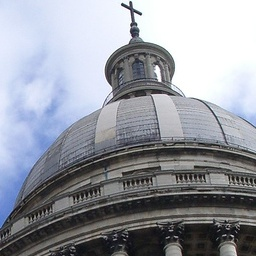
\includegraphics[width=0.16\textwidth]{./fig/NYUD2/images/3.jpg}
    \includegraphics[width=0.16\textwidth]{./fig/NYUD2/images/5.jpg}
    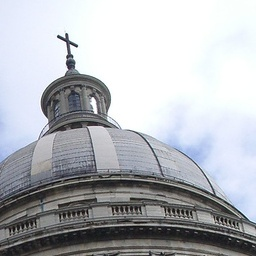
\includegraphics[width=0.16\textwidth]{./fig/NYUD2/images/6.jpg}
    \includegraphics[width=0.16\textwidth]{./fig/NYUD2/images/7.jpg}
    \includegraphics[width=0.16\textwidth]{./fig/NYUD2/images/8.jpg}
    \includegraphics[width=0.16\textwidth]{./fig/NYUD2/images/11.jpg} \\
     
\rotatebox{90}{Ground-truth}    
     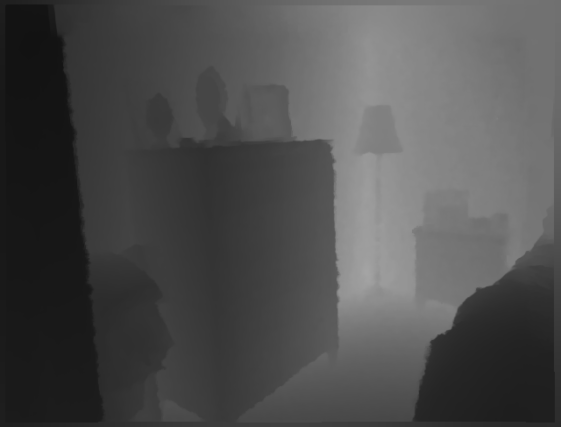
\includegraphics[width=0.16\textwidth]{./fig/NYUD2/gt/3.png}
     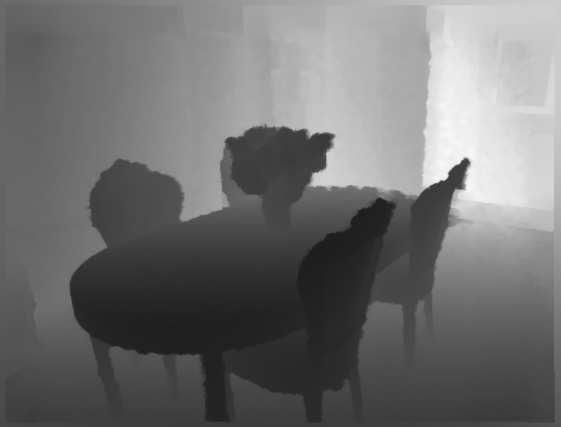
\includegraphics[width=0.16\textwidth]{./fig/NYUD2/gt/5.png}
     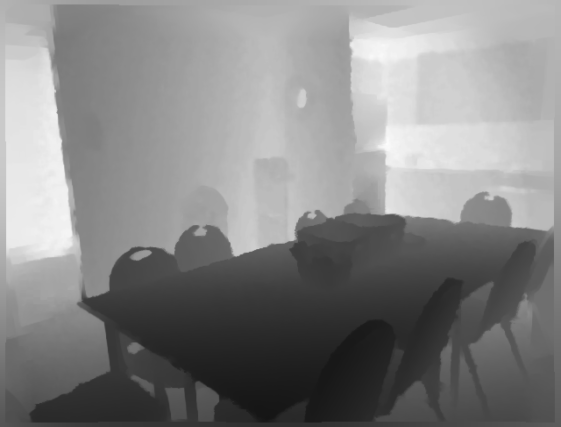
\includegraphics[width=0.16\textwidth]{./fig/NYUD2/gt/6.png}
     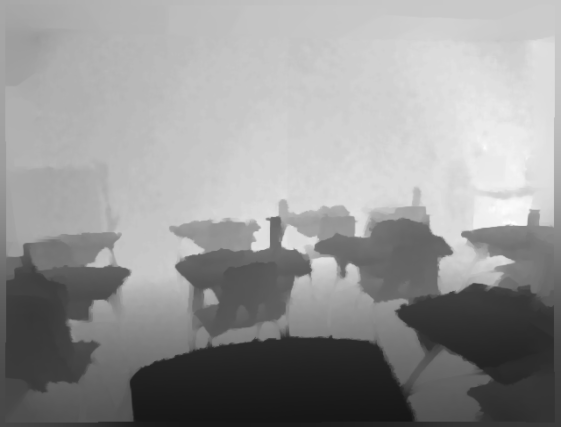
\includegraphics[width=0.16\textwidth]{./fig/NYUD2/gt/7.png}
     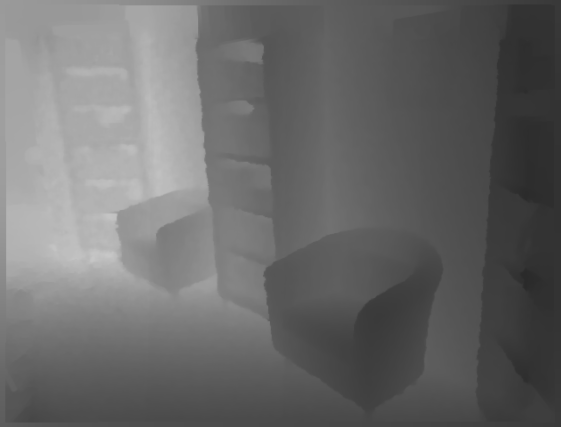
\includegraphics[width=0.16\textwidth]{./fig/NYUD2/gt/8.png}
     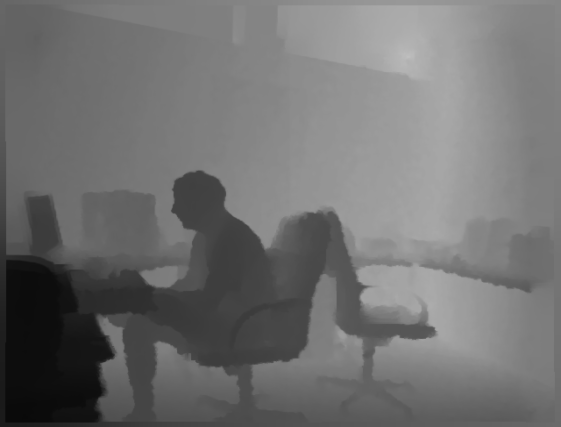
\includegraphics[width=0.16\textwidth]{./fig/NYUD2/gt/11.png} \\
     
\rotatebox{90}{Eigen \etal \cite{dcnn_nips14}}     
     
\includegraphics[width=0.16\textwidth]{./fig/NYUD2/nips14/3.png} 
     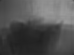
\includegraphics[width=0.16\textwidth]{./fig/NYUD2/nips14/5.png} 
     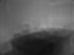
\includegraphics[width=0.16\textwidth]{./fig/NYUD2/nips14/6.png}
     \includegraphics[width=0.16\textwidth]{./fig/NYUD2/nips14/7.png} 
     \includegraphics[width=0.16\textwidth]{./fig/NYUD2/nips14/8.png} 
     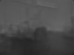
\includegraphics[width=0.16\textwidth]{./fig/NYUD2/nips14/11.png}  \\

\rotatebox{90}{Ours (fine-tune)}     
     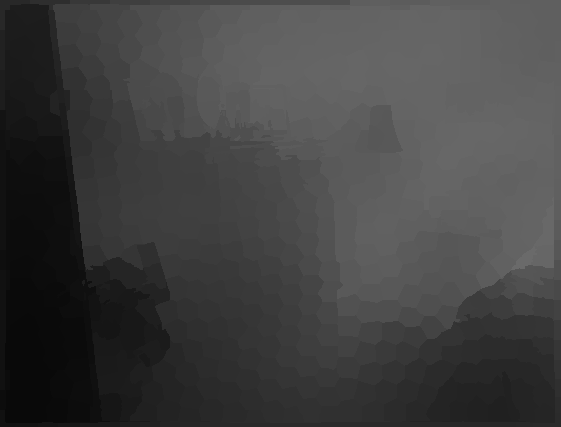
\includegraphics[width=0.16\textwidth]{./fig/NYUD2/ours_ft/3.png}  
     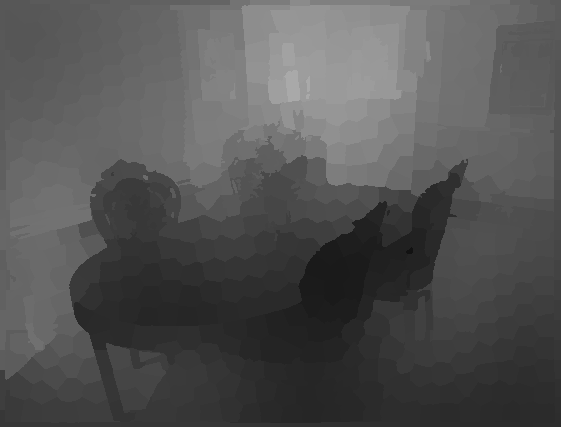
\includegraphics[width=0.16\textwidth]{./fig/NYUD2/ours_ft/5.png}
     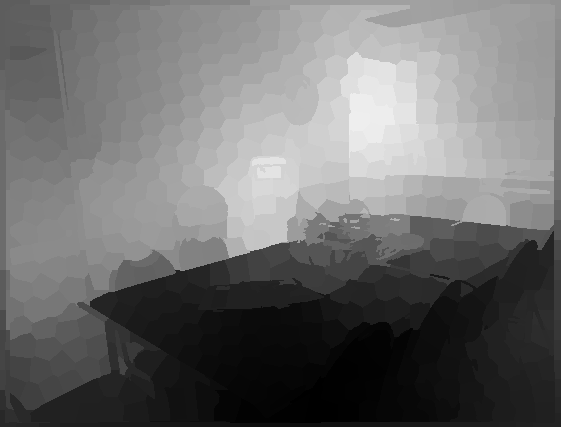
\includegraphics[width=0.16\textwidth]{./fig/NYUD2/ours_ft/6.png}
     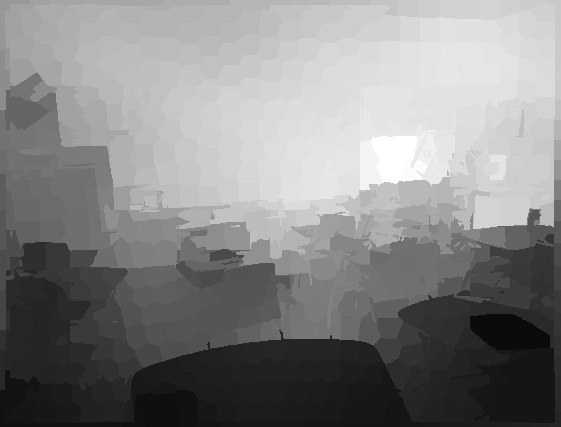
\includegraphics[width=0.16\textwidth]{./fig/NYUD2/ours_ft/7.png}    
     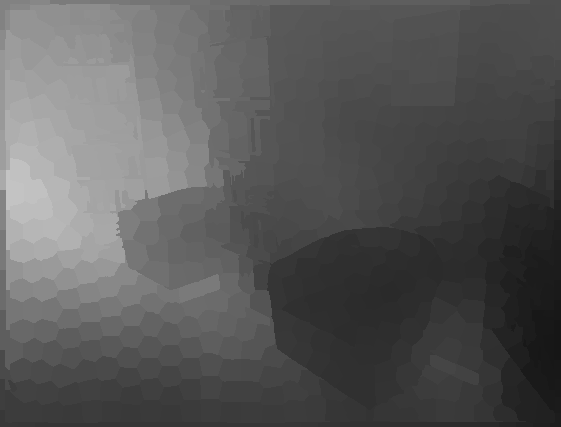
\includegraphics[width=0.16\textwidth]{./fig/NYUD2/ours_ft/8.png}
     \includegraphics[width=0.16\textwidth]{./fig/NYUD2/ours_ft/11.png}  \\   
\end{tabular}  
}   
\caption{Examples of qualitative comparisons on the NYUD2 dataset (Best viewed on screen).
Our method yields visually better predictions with sharper transitions, aligning to local details.
%
 }  \label{fig:nyud2}
\end{figure*}
























\begin{table*} [t] \center
\resizebox{.65\linewidth}{!} {
\begin{tabular}{ | l |  c  c  c | c  c  c |}
\hline 
\multirow{3}{*}{{{Method}}} &\multicolumn{3}{c|}{Error} &\multicolumn{3}{c|}{Accuracy} \\
&\multicolumn{3}{c|}{(lower is better)} &\multicolumn{3}{c|}{(higher is better)} \\
\cline{2-7}
&rel &log10 &rms &$\delta < 1.25$ &$\delta < 1.25^2$ &$\delta < 1.25^3$  \\
\hline
Make3d \cite{make3d_pami09}		  &0.349  &-  &1.214	&0.447	&0.745	&0.897 \\
DepthTransfer \cite{depthTransfer_pami14}	&0.35 	&0.131	&1.2		&- &- &-	 \\
Discrete-continuous \crf \cite{Miaomiao_cvpr14}	    &0.335	&0.127	&1.06 &- &- &-	 \\
Ladicky \etal \cite{Ladicky_cvpr14}		&- &- &-	&0.542	&0.829	&0.941  \\
Eigen \etal \cite{dcnn_nips14}      &\textbf{0.215}	&-	&0.907	&0.611	&\textbf{0.887}	&\textbf{0.971} \\
\hline
%
%
Ours (pre-train) &0.257	 &0.101	  &0.843  	&0.588   	&0.868	&0.961  \\
Ours (fine-tune)    &0.230	 &\textbf{0.095} 	 &\textbf{0.824}  &\textbf{0.614} 	 &0.883	 &\textbf{0.971} \\
\hline
\end{tabular}
}
\caption{Result comparisons on the NYU v2 dataset. 
Our method performs the best in most cases.
Kindly note that the results of Eigen \etal \cite{dcnn_nips14} are obtained by using extra training data (in the millions in total) while ours are obtained using the standard training set.} \label{tab:nyud2}
\end{table*}












\begin{table}
\center
\resizebox{1\linewidth}{!} {
\begin{tabular}{ | l |  c  c  c | c  c  c |}
\hline 
\multirow{3}{*}{{{Method}}} &\multicolumn{3}{c|}{Error} &\multicolumn{3}{c|}{Accuracy} \\
&\multicolumn{3}{c|}{(lower is better)} &\multicolumn{3}{c|}{(higher is better)} \\
\cline{2-7}
&rel &log10 &rms &$\delta < 1.25$ &$\delta < 1.25^2$ &$\delta < 1.25^3$  \\
\hline
%
SVR  &0.313	&0.128	&1.068	&0.490	&0.787	&0.921 \\
SVR (smooth) &0.290	 &0.116	&0.993	&0.514	&0.821	&0.943\\
Ours (unary only)  &0.295 	 &0.117 	 &0.985   &0.516 	 &0.815 	 &0.938  \\ 
%
Ours (pre-train) &0.257	 &0.101	  &0.843  	&0.588   	&0.868	&0.961  \\
Ours (fine-tune)  &\textbf{0.230} 	 &\textbf{0.095} 	 &\textbf{0.824}  &\textbf{0.614} 	 &\textbf{0.883} 	 &\textbf{0.971}\\    
\hline
\end{tabular}
}
\caption{Baseline comparisons on the NYU v2 dataset. 
Our method with the whole network training performs the best.
} \label{tab:anal_nyud2}
\end{table}










\begin{table}
\center
\resizebox{0.90\linewidth}{!} {
\begin{tabular}{ | l |  c  c  c | c  c  c |}
\hline 
\multirow{3}{*}{{{Method}}} &\multicolumn{3}{c|}{Error (C1)} &\multicolumn{3}{c|}{Error (C2)} \\
&\multicolumn{3}{c|}{(lower is better)} &\multicolumn{3}{c|}{(lower is better)} \\
\cline{2-7}
&rel &log10 &rms  &rel &log10 &rms  \\
\hline
%
SVR  &0.433	&0.158	&8.93  &0.429	&0.170	&15.29  \\
SVR (smooth) &0.380	&0.140	&\textbf{8.12}  &0.384	&0.155	&15.10 \\
Ours (unary only) &0.366 	 &0.137 	 &8.63  &0.363 	 &0.148 	 &14.41 \\
%
Ours (pre-train) &0.331	 &0.127	 &8.82  &0.324	&0.134	&13.29 \\
Ours (fine-tune)   &\textbf{0.314} &\textbf{0.119} &8.60 &\textbf{0.307} &\textbf{0.125} &\textbf{12.89} \\ 
%
\hline
\end{tabular}
}
\caption{Baseline comparisons on the Make3D dataset. 
Our method with the whole network training performs the best.
} \label{tab:anal_make3d}
\end{table}











\begin{table*} \center
\resizebox{.55\linewidth}{!} {
\begin{tabular}{ | l |  c  c  c | c  c  c |}
\hline 
\multirow{2}{*}{{{Method}}} &\multicolumn{3}{c|}{Error (C1)} &\multicolumn{3}{c|}{Error (C2)} \\
&\multicolumn{3}{c|}{(lower is better)} &\multicolumn{3}{c|}{(lower is better)} \\
\cline{2-7}
&rel &log10 &rms  &rel &log10 &rms  \\
\hline
Make3d \cite{make3d_pami09}		  &-  &-  &- 	&0.370	&0.187  &-  \\
Semantic Labelling \cite{Liu_cvpr12}  &-  &-  &- 	&0.379 &0.148 &- \\
DepthTransfer \cite{depthTransfer_pami14}	&0.355	&0.127	&9.20  &0.361	  &0.148	  &15.10 \\
Discrete-continuous \crf \cite{Miaomiao_cvpr14}	    &0.335	&0.137	&9.49  &0.338	  &0.134	 &\textbf{12.60}  \\
\hline
%
Ours (pre-train) &0.331	 &0.127	 &8.82  &0.324	&0.134	&13.29 \\
Ours (fine-tune)  &\textbf{0.314} &\textbf{0.119} &\textbf{8.60} &\textbf{0.307} &\textbf{0.125} &12.89 \\
%
\hline
\end{tabular}
}
\caption{Result comparisons on the Make3D dataset. 
Our method performs the best.
Kindly note that the C2 errors of the Discrete-continuous \crf \cite{Miaomiao_cvpr14} are reported with an ad-hoc post-processing step (train a classifier to label sky pixels and set the corresponding regions to the maximum depth).} \label{tab:make3d}
\end{table*}










\begin{figure*} [t] \center
\resizebox{.80\linewidth}{!} {
\begin{tabular}{cccccc}
\rotatebox{90}{Test image}
	\includegraphics[width=0.12\textwidth]{./fig/Make3D/image/58.jpg}
	\includegraphics[width=0.12\textwidth]{./fig/Make3D/image/60.jpg}
	\includegraphics[width=0.12\textwidth]{./fig/Make3D/image/9.jpg}
	\includegraphics[width=0.12\textwidth]{./fig/Make3D/image/8.jpg}
	\includegraphics[width=0.12\textwidth]{./fig/Make3D/image/81.jpg}
	\includegraphics[width=0.12\textwidth]{./fig/Make3D/image/5.jpg} \\
	
	
\rotatebox{90}{Ground-truth}
	\includegraphics[width=0.12\textwidth]{./fig/Make3D/gt/58.png}
	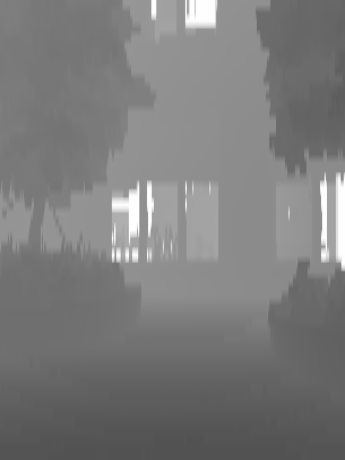
\includegraphics[width=0.12\textwidth]{./fig/Make3D/gt/60.png}
	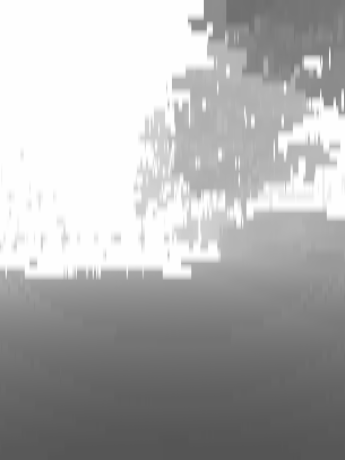
\includegraphics[width=0.12\textwidth]{./fig/Make3D/gt/9.png}
	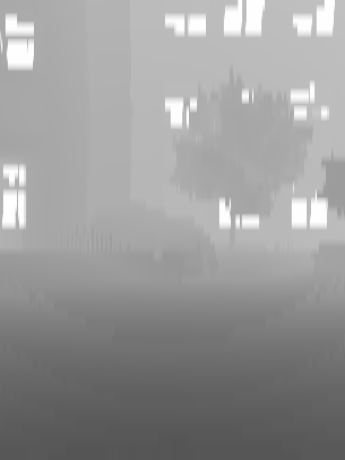
\includegraphics[width=0.12\textwidth]{./fig/Make3D/gt/8.png}
	\includegraphics[width=0.12\textwidth]{./fig/Make3D/gt/81.png}
	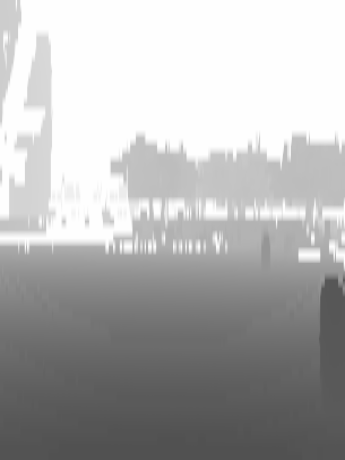
\includegraphics[width=0.12\textwidth]{./fig/Make3D/gt/5.png} \\
	
	
\rotatebox{90}{Ours (unary only)}
	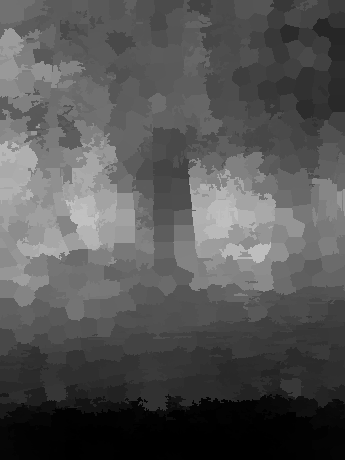
\includegraphics[width=0.12\textwidth]{./fig/Make3D/unary/58.png}
	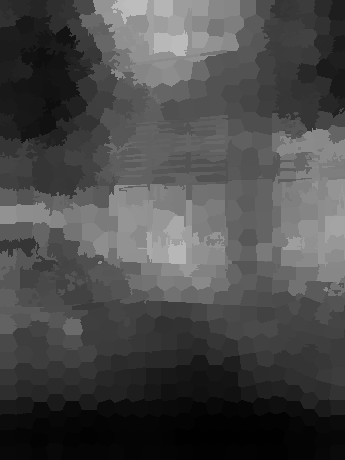
\includegraphics[width=0.12\textwidth]{./fig/Make3D/unary/60.png}
	\includegraphics[width=0.12\textwidth]{./fig/Make3D/unary/9.png}
	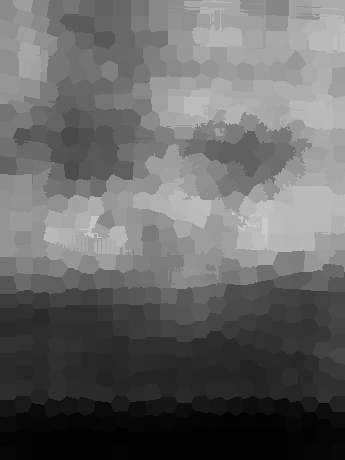
\includegraphics[width=0.12\textwidth]{./fig/Make3D/unary/8.png}
	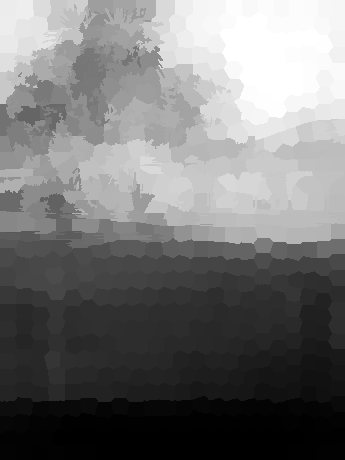
\includegraphics[width=0.12\textwidth]{./fig/Make3D/unary/81.png}
	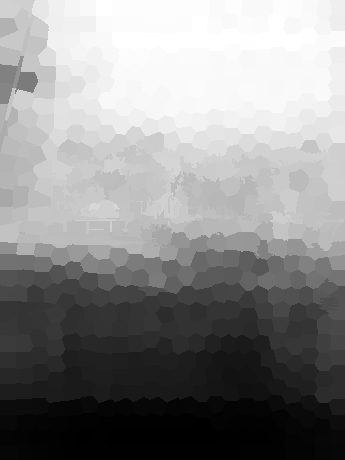
\includegraphics[width=0.12\textwidth]{./fig/Make3D/unary/5.png} \\
	

%
%
%
%
%
%
%
	
	
\rotatebox{90}{Ours (fine-tune)}
	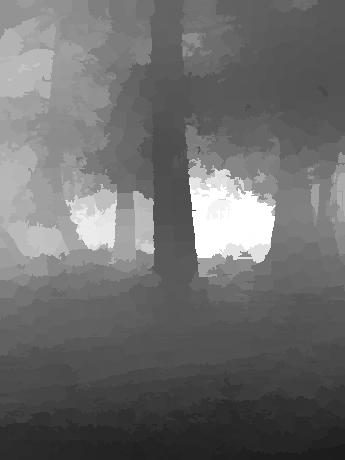
\includegraphics[width=0.12\textwidth]{./fig/Make3D/ccnf_struct_ft/58.png}
	\includegraphics[width=0.12\textwidth]{./fig/Make3D/ccnf_struct_ft/60.png}
	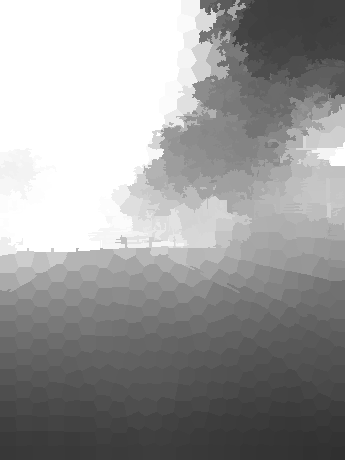
\includegraphics[width=0.12\textwidth]{./fig/Make3D/ccnf_struct_ft/9.png}
	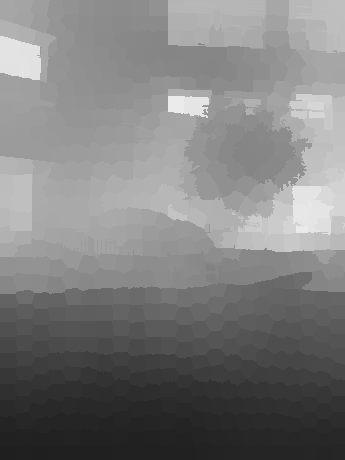
\includegraphics[width=0.12\textwidth]{./fig/Make3D/ccnf_struct_ft/8.png}
	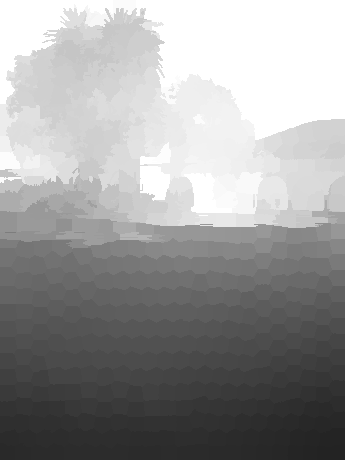
\includegraphics[width=0.12\textwidth]{./fig/Make3D/ccnf_struct_ft/81.png}
	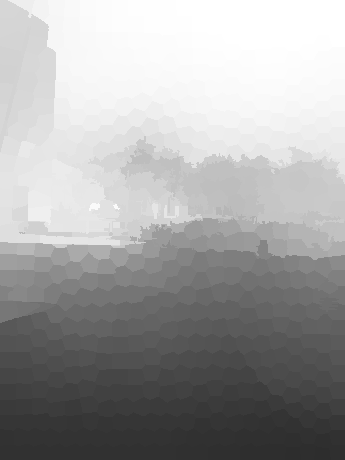
\includegraphics[width=0.12\textwidth]{./fig/Make3D/ccnf_struct_ft/5.png} \\	
 \end{tabular}      
 } 
\caption{Examples of depth predictions on the Make3D dataset (Best viewed on screen).
The unary only model gives rather coarse predictions, with blurry boundaries and segments. In contrast, our full model with pairwise smoothness yields much better predictions.
}  \label{fig:nmake3d}
\end{figure*}































\section{Experiments}


We evaluate on two popular datasets which are available online: the NYU v2 Kinect dataset \cite{nyud2_eccv12} and the Make3D range image dataset \cite{make3d_pami09}. 
Several measures commonly used in prior works are applied here for quantitative evaluations:
\begin{itemize}
\vspace{-.12cm} \item
average relative error (rel): 
$\frac{1}{T} \sum_p \frac{|d_p^{gt} - d_p|}{d_p^{gt}} $;
\vspace{-.12cm} \item
root mean squared error (rms): 
$\sqrt{\frac{1}{T} \sum_p (d_p^{gt} - d_p)^2}$;
\vspace{-.12cm} \item
average $\log_{10}$ error (log10): \\
$\frac{1}{T} \sum_p | \log_{10}d_p^{gt} - \log_{10}d_p|$;
\vspace{-.12cm} \item
accuracy with threshold $thr$: \\
percentage ($\%$) of $d_p \; \; \st \max (\frac{d_p^{gt}}{d_p}, \frac{d_p}{d_p^{gt}}) = \delta < thr$;
\end{itemize}
%
%
%
%
%
%
%
%
%
%
%
%
%
%
%
%
%
%
%
%
where $d_p^{gt}$ and $d_p$ are the ground-truth and predicted depths respectively at pixel indexed by $p$, and $T$ is the total number of pixels in all the evaluated images. 

We use SLIC \cite{slic_pami12} to segment the images into a set of non-overlapping superpixels. For each superpixel, we consider the image within a rectangular box centred on the centroid of the superpixel, which contains a large portion of its background surroundings. More specifically, we use a box size of 168$\times$168 pixels for the NYU v2 and $120 \times 120$ pixels for the Make3D dataset.
%
Following \cite{make3d_pami09,Liu_cvpr12,dcnn_nips14}, we transform the depths into log-scale before training.
%
As for baseline comparisons, we consider the following settings:
\begin{itemize}
\vspace{-.12cm} \item
SVR: We train a support vector regressor using the \cnn representations from the first 6 layers of Fig. \ref{fig:cnn_unary}; 
\vspace{-.12cm} \item
SVR (smooth): We add a smoothness term to the trained SVR during prediction by solving the inference problem in Eq. \eqref{eq:inf_solution}. As tuning multiple pairwise parameters is not straightforward, we only use color difference as the pairwise potential and choose the parameter $\beta$ by hand-tuning on a validation set;
\vspace{-.12cm} \item
Unary only: We replace the \crf loss layer in Fig. \ref{fig:cnn_ccrf} with a least-square regression layer (by setting the pairwise outputs $\pws_{pq}=0$, $p,q=1,...,n$), which degenerates to a deep regression model trained by SGD.
\end{itemize}
 



























\subsection{NYU v2: Indoor scene reconstruction}
The NYU v2 dataset consists of $1449$ RGBD images of indoor scenes, among which $795$ are used for training and 654 for test (we use the standard training/test split provided with the dataset).
Following \cite{Miaomiao_cvpr14}, we resize the images to $427 \times 561$ pixels 
before training.%


For a detailed analysis of our model, we first compare with the three baseline methods and report the results in Table \ref{tab:anal_nyud2}. 
From the table, several conclusions can be made: 1) When trained with only unary term, deeper network is beneficial for better performance, which is demonstrated by the fact that our unary only model outperforms the SVR model;
2) Adding smoothness term to the SVR or our unary only model helps improve the prediction accuracy;
3) Our method achieves the best performance by jointly learning the unary and the pairwise parameters in a unified deep \cnn framework. Moreover, fine-tuning the whole network yields further performance gain.
These well demonstrate the efficacy of our model.
%
%
%
























In Table \ref{tab:nyud2}, we compare our model with several popular state-of-the-art methods.  
As can be observed, our method outperforms classic methods like Make3d \cite{make3d_pami09}, DepthTransfer \cite{depthTransfer_pami14} with large margins. 
Most notably, our results are significantly better than that of \cite{Ladicky_cvpr14}, which jointly exploits depth estimation and semantic labelling. 
Comparing to the recent work of Eigen \etal \cite{dcnn_nips14}, our method generally performs on par.
Our method obtains significantly better result in terms of root mean square (rms) error.
%
%
 %
%
%
%
Kindly note that, to overcome overfit, they \cite{dcnn_nips14} have to collect millions of additional labelled images to train their model. One possible reason is that their method captures the absolute pixel location information and they probably need a very large training set to cover all possible pixel layouts.
In contrast, we only use the standard training sets ($795$) without any extra data,  
yet we achieve comparable or even better performance.
Fig. \ref{fig:nyud2} illustrates some qualitative evaluations of our method compared against Eigen \etal \cite{dcnn_nips14} (We download the predictions of \cite{dcnn_nips14} from the authors' website.). 
%
%
Compared to the predictions of \cite{dcnn_nips14},
our method yields more visually pleasant predictions with sharper transitions, aligning to local details.


%
%
%
%








%
%
%
%
%
%
%
%
%
%
%
%
%
%
%
%
%
%
%
%
%
%
%
%
%
%
%



























\subsection{Make3D: Outdoor scene reconstruction}
The Make3D dataset contains 534 images depicting outdoor scenes.
%
As pointed out in \cite{make3d_pami09,Miaomiao_cvpr14}, this dataset is with limitations: the maximum value of depths is 81m with far-away objects are all mapped to the one distance of $81$ meters. 
As a remedy, two criteria are used in \cite{Miaomiao_cvpr14} to report the prediction errors: ($C_1$) Errors are calculated only in the regions with the ground-truth depth less than $70$ meters; ($C_2$) Errors are calculated over the entire image.
We follow this protocol to report the evaluation results. 

Likewise, we first present the baseline comparisons in Table \ref{tab:anal_make3d}, from which similar conclusions can be drawn as in the NYU v2 dataset. 
We then show the detailed results compared with several state-of-the-art methods in Table \ref{tab:make3d}.  
As can be observed, our model with 
the whole network training
ranks the first in overall performance,
outperforming the compared methods by large margins.
 %
Kindly note that the C2 errors of \cite{Miaomiao_cvpr14} are reported with an ad-hoc post-processing step, which trains a classifier to label sky pixels and set the corresponding regions to the maximum depth.
In contrast, we do not employ any of those heuristics to refine our results, yet we achieve better results in terms of relative error. %
%
Some examples of qualitative  evaluations are shown in Fig. \ref{fig:nmake3d}.  
%
It is shown that our unary only model gives rather coarse predictions with blurry boundaries. 
By adding smoothness term, our model yields much better visualizations, which are close to ground-truth.
 %













